\documentclass{article}

% if you need to pass options to natbib, use, e.g.:
%     \PassOptionsToPackage{numbers, compress}{natbib}
% before loading neurips_2020

% ready for submission
% \usepackage{neurips_2020}

% to compile a preprint version, e.g., for submission to arXiv, add add the
% [preprint] option:
\usepackage[preprint]{neurips_2020}

% to compile a camera-ready version, add the [final] option, e.g.:
%     \usepackage[final]{neurips_2020}

% to avoid loading the natbib package, add option nonatbib:
%    \usepackage[nonatbib]{neurips_2020}

\usepackage[utf8]{inputenc} % allow utf-8 input
\usepackage[T1]{fontenc}    % use 8-bit T1 fonts
\usepackage{hyperref}       % hyperlinks
\usepackage{url}            % simple URL typesetting
\usepackage{booktabs}       % professional-quality tables
\usepackage{amsfonts}       % blackboard math symbols
\usepackage{nicefrac}       % compact symbols for 1/2, etc.
\usepackage{microtype}      % microtypography
\usepackage{graphicx}

\title{Formatting Instructions For NeurIPS 2020}

% The \author macro works with any number of authors. There are two commands
% used to separate the names and addresses of multiple authors: \And and \AND.
%
% Using \And between authors leaves it to LaTeX to determine where to break the
% lines. Using \AND forces a line break at that point. So, if LaTeX puts 3 of 4
% authors names on the first line, and the last on the second line, try using
% \AND instead of \And before the third author name.

\title{Towards Interpretable Dimensionality Reduction\\
	\large Mathematical Foundations of Machine Learning}

\author{Roberto Barroso-Luque \\
	\texttt{barrosoluquer@uchicago.edu}  \\
	The University of Chicago
	\AND
	Hana Passen\\
	\texttt{passen@uchicago.edu} \\
    The University of Chicago\\}
\begin{document}
\maketitle

\begin{abstract}{
Dimensionality reduction through singular value decomposition (SVD), principal components analysis (PCA), and other techniques is a computationally efficient way to eliminate redundant features without losing significant predictive power. However, these methods are fraught with interpretability challenges. We investigated two methods to derive interpretable results from dimensionality reduction: 1) using simple correlations between classically derived principal components and the original features; 2) modifying an algorithm described by Chipman and Gu to create “interpretable directions” and taking the correlation between those interpretable directions and the original features. We conducted a set of experiments to test the interpretability and the predictive accuracy of these methods on a range of datasets, to test performance on both continuous and categorical features. We find that simple correlation analysis of features and PC directions can provide researchers with some intuitive understanding of lower dimensional representations of their original feature space, while also providing a sufficiently robust predictive model. While other methods can increase the interpretability of the PC directions, losses in predictive power may make these methods unpopular for prediction and analysis.}  
\end{abstract}

\newpage
\section{Introduction}
Dimensionality reduction through SVD, principal components analysis, and other techniques is a computationally efficient method to project high dimensional data onto a lower-dimensional subspace. When used in classification problems, these methods allow us to reduce the feature space by orders of magnitude eliminating redundant features all without necessarily losing predictive power. However, this methodology is fraught with interpretability challenges. While the relative importance of the singular values can still be understood via their magnitudes, it is difficult to explain what common-sense meaning a large singular value represents in the original data set. Principal components are linear combinations of the original features of a data matrix, and correspond to directions of greatest variance within the data; there is therefore an opportunity to identify which combinations of features are most represented by each principal component vector. To this end, we explore different methodologies to gain insights into the relationship between the features of a data matrix and its reduced dimension space.

\section{Methodology}{

\subsection{Datasets}{We conducted experiments on four datasets. One dataset uses 13 variables, some continuous and categorical, to classify the presence of heart disease in a patient (hereafter referred to as the HD dataset). One dataset uses survey respondents’ answers to 54 questions to predict whether the respondent is divorced (hereafter referred to as the Divorce dataset). One dataset uses 19 player statistic continuous variables to predict whether NBA rookies remain in the NBA after 5 years (hereafter referred to as the NBA dataset). The final dataset uses 23 categorical features of mushrooms, in biologically-related clusters, to predict whether that mushroom is poisonous (hereafter, the mushroom dataset).}


\subsection{Data Pre-processing}{In some cases, we preprocessed our data by eliminating categorical variables, and normalizing continuous variables. We subtracted the mean from each column and divided by the standard deviation to achieve unit variance across all features. In other cases, when examining categorical data, we created dummy variables for each of the categories. Finally, we split the data into training and testing sets, with 80\% of the data in the training set and 20\% in the testing set. }


\subsection{Correlation Analysis}{To implement correlation analysis between the original features and the principal component vectors, we first decomposed the matrix using the full singular value decomposition. The spectrum of the feature space was then used to determine the most important of the components (Figure 1). All subsequent analysis performed was done using the most important principal components based on the result from the decomposition. Once the most important principal component vectors were identified, the pearson r coefficient was calculated between the PCA vectors and each individual feature in the original dataset. The absolute magnitudes of the correlation coefficients were then compared to determine the original features most closely related to each principal component vector.}


\subsection{Interpretable Directions}{Chipman and Gu describe a complex algorithm based on a principle of homogeneity between the original features.To provide a less cumbersome and more intuitive solution, we modified their algorithm to produce a simplified version of their “interpretable directions” (ID). 
The modified algorithm described by Chipman et al. is as follows: 
For each principal component vector, for every value of k from 1 to the number of non-zero entries in that vector, identify the k entries with the largest absolute values. Set those entries to positive or negative 1 (based on the sign of the entry in the principal component vector) divided by the square root of k. Set all the other entries in the vector equal to zero. Finally, compute a measure of similarity between the new vector and the principal component vector. The vector that is the closest to the original principal component vector is the new ID vector. We computed squared distance - rather than cosine similarity as described by Chipman and Gu - as the measure of similarity between vectors. 	
In general, this method sets variables that may be correlated with each other to another variable of the same magnitude, and tests the correlation between these homogenized direction vectors and the original principal component vectors. While Chipman and Gu only explore this method with respect to continuous variables, we extended their method to also test its performance on categorical features.
}


\subsection{Prediction}{We used linear classification models to predict the target variable based on reducing our data to the most important PCs and the corresponding most important IDs, and compared their prediction accuracy. To project the data into the lower dimensional subspace, we used a singular value decomposition. From the decomposition we multiplied the most important singular values with their respective left singular vectors to compute a lower dimensional representation of the original space. Once generated, we compared prediction results on the respective target values by either training our least squares classifier with samples from the original dataset or using samples from the lower dimensional representation of this space. For both procedures we used the same test and training set to fairly compare accuracy results. (Table 4)}
}

\section{Discussion and Findings}{
\subsection{Interpretability of Principal Components}{
The first method of correlation mapping between features and PCs provides some intuition into what a PC direction represents. We are able to identify, in absolute magnitude terms, which of the original features are most highly correlated with a given PC direction (Table 2) and take common-sense interpretations of what those highly correlated features represent.
The second method, using Chipman and Gu’s algorithm to create IDs showed mixed results. Using the NBA dataset, comprised solely of continuous features, the IDs did add to the intuitive understanding of the variables correlated with the direction vectors. In the simple correlation between the PCs and the original features, the most correlated features were the number of offensive rebounds and total rebounds, followed by blocks and 3 points made. This tells us which statistics may be important, but they do not draw a unified picture of the most important player behavior. However, when taking the correlations of the IDs and the original features, the most highly correlated features changed.(Table 3) While offensive rebounds was still the most highly correlated feature, the three-pointers made and three-point percentage were the next most highly correlated. These three features are all offensive gameplay features, which may suggest that the first ID is the "offensive gameplay" direction. And indeed, some of the next most highly correlated features in that ID are three point attempts, field goal percent, and total rebounds. This direction, in which offensive behavior is all highly correlated, does appear to be more interpretable than the original PC vector, which included blocks (a defensive statistic).
When applied to categorical features in the mushroom dataset, the Chipman and Gu method had more mixed results. The features most highly correlated with the original PC mappings were 1) those features that represented instances of a binary category (bruises and stalk shape).
Using the Heart Disease dataset, which combined continuous and categorical features, there were very few differences between the simple feature correlations with the original PCA directions and the feature correlations with the IDs. When using only continuous data, the same original features were highly correlated with both the PCs and IDs - while there were some changes in the magnitude of those correlations, the distribution and difference between the correlations was not particularly different. Equally, when extending Chipman and Gu’s method to categorical features, the correlations between the features and the PCs and the IDs also remained similar in magnitude and proportion to one another.
}

\subsection{Predictive Accuracy}{
One motivation for this work is to make classifications based on a lower-dimensional representation of our original data. Using the methodology described above, we made predictions on various datasets using the three models. 
When making predictions on continuous data (the NBA dataset), we see a drop in accuracy between the classical principal components analysis and prediction using the IDs. In this case, from a least squares classification error of .67, classification using the first two PCs resulted in an error of .56, while classification using the first two IDs resulted in an error of .41. The ID-reduced dimensionality performs significantly less well than least squares prediction, while PC-reduced dimensionality does somewhat better. (Table 4)
When making predictions on categorical data (the mushrooms dataset), we found very slight differences between the prediction accuracy using least squares, and the prediction accuracy using reduced-dimension PCs and IDs. In this case, the least squares error was .48, while the error for both the other methods was .47. We would need to test these results on more categorical datasets, but this suggests at least preliminarily that we lose little predictive power when reducing categorical data dimensionality to a few key PC or ID directions. 

When making predictions on the Heart Disease dataset, we found mixed results. With the data reduced to only continuous features, there was a small decrease in prediction accuracy from .72 using the least squares model to .70 using a single principle component for prediction, while there was a large decrease to .40 using a single “interpretable direction”. In this case, we see only a small loss in predictive power from least squares to PC prediction, with some gains in interpretability. However, when including the continuous and dummy categorical features, the results were quite different. In this case, while the least squares classifier had an accuracy of .59, classical PCA had an accuracy of .77 while the "interpretable directions" had an accuracy of .70, suggesting that the correlation between variables created issues for least squares classification, while not presenting similar challenges for PC prediction. These results are unexpected - given that principal component vectors are linear combinations of the original features, a lower dimensional representation of a dataset should have higher predictive power than the full dataset. We attribute this unexpected result to chance. We performed only a single train-test split on our data. Our speculation is that had we followed an iterative algorithm for evaluation such as K-fold cross validation the lower dimensional features would converge at a higher average error when compared to making predictions using the full dataset.
}

\subsection{Conclusion}{
Correlation analysis can be used to determine some intuition about the variance in a dataset represented by a PC direction. In some cases, particularly for continuous variables, we can use methods like Chipman and Gu’s (which applies a homogeneity principle to the data) to produce IDs that approximate a PC direction, to improve interpretability of the data. In no cases, however, were Chipman and Gu’s ID vectors better at predicting than classically derived PCs. The small improvements in interpretability may not be worth the sometimes large losses in predictive power between the two models - the interpretability of PCs based on correlation mapping may give a sufficient insight into the area of greatest variance without sacrificing predictive power.} 
}

\begin{figure}
	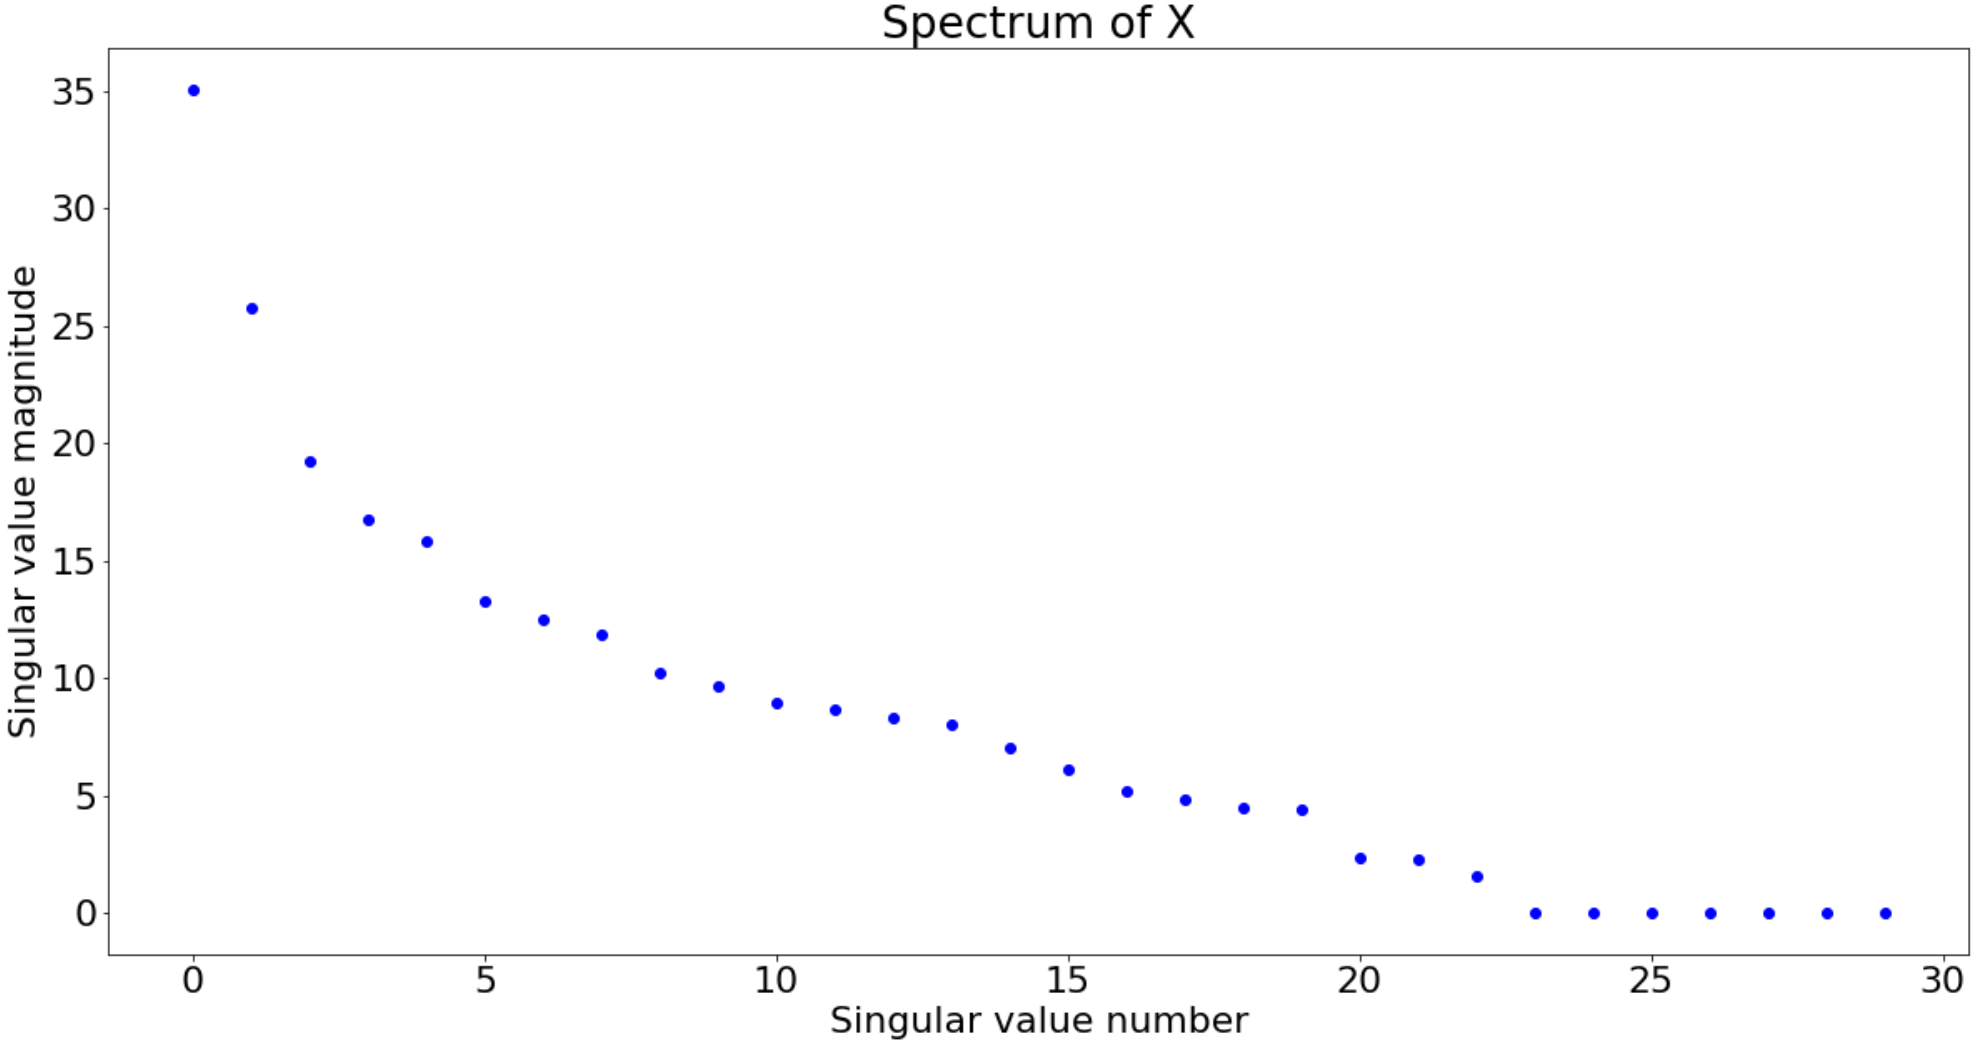
\includegraphics[width=\linewidth]{spectrumHD.png}
	\caption{Example of Spectrum from SVD of Heart Disease Data.}
\end{figure}


\begin{table}
  \caption{Number of principal component vectors and ratio of variance explained.}
  \centering
  \begin{tabular}{lll}
    \toprule
    \midrule
    Dataset     & PCA Vectors Used       & Variance Explained \\
    \midrule
    \midrule
    Heart Disease(continuous only) & 1 & .25     \\
    \midrule
    Heart Disease & 2 & .41     \\
    \midrule
    Divorce     & 1 & .31    \\
    \midrule
    NBA Rookies     & 2   & .55 \\
    \midrule
    Mushrooms     & 1   & .34 \\
    \bottomrule
  \end{tabular}
\end{table}

\begin{table}
	\caption{ Original features with highest correlation to chosen principal component vectors.}
	\centering
	\begin{tabular}{lll}
    \toprule
	\midrule
	Dataset     & Original feature (label)     & Correlation to PC vector(R2) \\
	\midrule
	\midrule
	Heart Disease(continuous only) & Thalach (max heart rate) & .89     \\
	\midrule
	Heart Disease & Age & .69     \\
	\midrule
	Divorce     & Atr7  & .45    \\
	\midrule
	NBA Rookies     & Offensive Rebounds   & .80 \\
	\midrule
	Mushrooms     & Stalk Shape-enlarging and shape-tapering   & .58 \\
	\bottomrule
	\end{tabular}
\end{table}

\begin{table}
	\caption{Original features with highest correlation to chosen “interpretable direction” vectors }
	\centering
	\begin{tabular}{lll}
		\toprule
		\midrule
		Dataset     & Original feature (label)     & Correlation to ID vectors(R2) \\
		\midrule
		\midrule
		Heart Disease(continuous only) & Thalach (max heart rate) & .79     \\
		\midrule
		Heart Disease & Oldpeak & .58     \\
		\midrule
		NBA Rookies     & Offensive Rebounds   & .68 \\
		\midrule
		Mushrooms  & Odor-musty, ring-type-none, ring-number-none   & .88 \\
		\bottomrule
	\end{tabular}
\end{table}


\begin{table}
	\caption{ Prediction accuracy using PCs, IDs, and original feature space}
	\centering
	
	\begin{tabular}{llll}
		\toprule
		\midrule	
		Dataset     & Full features space (Least Squares) & PCA Least Squares & ID Least Squares \\
		\midrule
		\midrule
		Heart Disease(continuous only) & .72 & .70 & .40    \\
		\midrule
		Heart Disease*  & .59 & .77 & .70    \\
		\midrule
		Divorce     & 1.00 & .50 & NA  \\
		\midrule
		NBA Rookies   & .67 & .56 & .41    \\
		\midrule
		Mushrooms     & .48 & .47 & .47    \\
		\bottomrule
	\end{tabular}
Note: For all classification tasks the feature matrix was broken into 80\% training set and 20\% testing set. 
Accuracy shown in the table is based on the training set.
*These errors are not what we expected. See findings section.
\end{table}




\section{References}\label{sec_ref}

[1] Chipman H. \& Gu H. (2006): Interpretable dimension reduction. 
{\it Journal of Applied Statistics}

[2] Ding J. , Condon A. \& P.Shah S. (2018). Interpretable dimensionality reduction \\ of single cell transcriptome data with deep generative models. 
{\it Nature Communications}

[3]Hosseini B. \& Hammer B (2019): Interpretable Discriminative Dimensionality Reduction \\ and Feature Selection on the Manifold.
{\it BiorXiv}


\end{document}
